\documentclass{article}\usepackage[]{graphicx}\usepackage[]{color}
% maxwidth is the original width if it is less than linewidth
% otherwise use linewidth (to make sure the graphics do not exceed the margin)
\makeatletter
\def\maxwidth{ %
  \ifdim\Gin@nat@width>\linewidth
    \linewidth
  \else
    \Gin@nat@width
  \fi
}
\makeatother

\definecolor{fgcolor}{rgb}{0.345, 0.345, 0.345}
\newcommand{\hlnum}[1]{\textcolor[rgb]{0.686,0.059,0.569}{#1}}%
\newcommand{\hlstr}[1]{\textcolor[rgb]{0.192,0.494,0.8}{#1}}%
\newcommand{\hlcom}[1]{\textcolor[rgb]{0.678,0.584,0.686}{\textit{#1}}}%
\newcommand{\hlopt}[1]{\textcolor[rgb]{0,0,0}{#1}}%
\newcommand{\hlstd}[1]{\textcolor[rgb]{0.345,0.345,0.345}{#1}}%
\newcommand{\hlkwa}[1]{\textcolor[rgb]{0.161,0.373,0.58}{\textbf{#1}}}%
\newcommand{\hlkwb}[1]{\textcolor[rgb]{0.69,0.353,0.396}{#1}}%
\newcommand{\hlkwc}[1]{\textcolor[rgb]{0.333,0.667,0.333}{#1}}%
\newcommand{\hlkwd}[1]{\textcolor[rgb]{0.737,0.353,0.396}{\textbf{#1}}}%
\let\hlipl\hlkwb

\usepackage{framed}
\makeatletter
\newenvironment{kframe}{%
 \def\at@end@of@kframe{}%
 \ifinner\ifhmode%
  \def\at@end@of@kframe{\end{minipage}}%
  \begin{minipage}{\columnwidth}%
 \fi\fi%
 \def\FrameCommand##1{\hskip\@totalleftmargin \hskip-\fboxsep
 \colorbox{shadecolor}{##1}\hskip-\fboxsep
     % There is no \\@totalrightmargin, so:
     \hskip-\linewidth \hskip-\@totalleftmargin \hskip\columnwidth}%
 \MakeFramed {\advance\hsize-\width
   \@totalleftmargin\z@ \linewidth\hsize
   \@setminipage}}%
 {\par\unskip\endMakeFramed%
 \at@end@of@kframe}
\makeatother

\definecolor{shadecolor}{rgb}{.97, .97, .97}
\definecolor{messagecolor}{rgb}{0, 0, 0}
\definecolor{warningcolor}{rgb}{1, 0, 1}
\definecolor{errorcolor}{rgb}{1, 0, 0}
\newenvironment{knitrout}{}{} % an empty environment to be redefined in TeX

\usepackage{alltt}
\usepackage[]{graphicx}
\usepackage[]{color}
\usepackage[colorlinks=true,linkcolor=blue]{hyperref}
% maxwidth is the original width if it is less than linewidth
% otherwise use linewidth (to make sure the graphics do not exceed the margin)


\makeatletter
\def\maxwidth{ %
  \ifdim\Gin@nat@width>\linewidth
    \linewidth
  \else
    \Gin@nat@width
  \fi
}
\makeatother

\definecolor{fgcolor}{rgb}{0.345, 0.345, 0.345}
%\newcommand{\hlnum}[1]{\textcolor[rgb]{0.686,0.059,0.569}{#1}}%
%\newcommand{\hlstr}[1]{\textcolor[rgb]{0.192,0.494,0.8}{#1}}%
%\newcommand{\hlcom}[1]{\textcolor[rgb]{0.678,0.584,0.686}{\textit{#1}}}%
%\newcommand{\hlopt}[1]{\textcolor[rgb]{0,0,0}{#1}}%
%\newcommand{\hlstd}[1]{\textcolor[rgb]{0.345,0.345,0.345}{#1}}% 
%\newcommand{\hlkwa}[1]{\textcolor[rgb]{0.161,0.373,0.58}{\textbf{#1}}}%
%\newcommand{\hlkwb}[1]{\textcolor[rgb]{0.69,0.353,0.396}{#1}}%
%\newcommand{\hlkwc}[1]{\textcolor[rgb]{0.333,0.667,0.333}{#1}}%
%\newcommand{\hlkwd}[1]{\textcolor[rgb]{0.737,0.353,0.396}{\textbf{#1}}}%
%\let\hlipl\hlkwb

\usepackage{framed}
\makeatletter

%\newenvironment{kframe}{%
% \def\at@end@of@kframe{}%
% \ifinner\ifhmode%
%  \def\at@end@of@kframe{\end{minipage}}%
%  \begin{minipage}{\columnwidth}%
% \fi\fi%
% \def\FrameCommand##1{\hskip\@totalleftmargin \hskip-\fboxsep
% \colorbox{shadecolor}{##1}\hskip-\fboxsep
     % There is no \\@totalrightmargin, so:
%     \hskip-\linewidth \hskip-\@totalleftmargin \hskip\columnwidth}%
% \MakeFramed {\advance\hsize-\width
%   \@totalleftmargin\z@ \linewidth\hsize
%   \@setminipage}}%
% {\par\unskip\endMakeFramed%
% \at@end@of@kframe}
%\makeatother

\definecolor{shadecolor}{rgb}{.97, .97, .97}
\definecolor{messagecolor}{rgb}{0, 0, 0}
\definecolor{warningcolor}{rgb}{1, 0, 1}
\definecolor{errorcolor}{rgb}{1, 0, 0}
%\newenvironment{knitrout}{}{} % an empty environment to be redefined in TeX

\usepackage{alltt}
\usepackage{listings}

\definecolor{mygreen}{rgb}{0,0.6,0}
\definecolor{mygray}{rgb}{0.5,0.5,0.5}
\definecolor{mymauve}{rgb}{0.58,0,0.82}

\lstset{ 
  backgroundcolor=\color{white},   % choose the background color; you must add \usepackage{color} or \usepackage{xcolor}; should come as last argument
  basicstyle=\footnotesize,        % the size of the fonts that are used for the code
  breakatwhitespace=false,         % sets if automatic breaks should only happen at whitespace
  breaklines=true,                 % sets automatic line breaking
  captionpos=,                    % sets the caption-position to bottom
  commentstyle=\color{mygreen},    % comment style
  deletekeywords={...},            % if you want to delete keywords from the given language
  escapeinside={\%*}{*)},          % if you want to add LaTeX within your code
  extendedchars=true,              % lets you use non-ASCII characters; for 8-bits encodings only, does not work with UTF-8
  firstnumber=1,                % start line enumeration with line 1000
  frame=single,	                   % adds a frame around the code
  keepspaces=true,                 % keeps spaces in text, useful for keeping indentation of code (possibly needs columns=flexible)
  keywordstyle=\color{blue},       % keyword style
  language=Python,                 % the language of the code
  morekeywords={*,...},            % if you want to add more keywords to the set
  numbers=left,                    % where to put the line-numbers; possible values are (none, left, right)
  numbersep=5pt,                   % how far the line-numbers are from the code
  numberstyle=\tiny\color{mygray}, % the style that is used for the line-numbers
  rulecolor=\color{black},         % if not set, the frame-color may be changed on line-breaks within not-black text (e.g. comments (green here))
  showspaces=false,                % show spaces everywhere adding particular underscores; it overrides 'showstringspaces'
  showstringspaces=false,          % underline spaces within strings only
  showtabs=false,                  % show tabs within strings adding particular underscores
  stepnumber=1,                    % the step between two line-numbers. If it's 1, each line will be numbered
  stringstyle=\color{mymauve},     % string literal style
  tabsize=2,	                   % sets default tabsize to 2 spaces
  title=\lstname                   % show the filename of files included with \lstinputlisting; also try caption instead of title
}
\IfFileExists{upquote.sty}{\usepackage{upquote}}{}
\begin{document}

\section{Introduction}

\subsection{How is particulate matter analyzed?}

The PM sensor has several components to measure the particles in the air -- remember, we don't know what the make up of these particles might be -- but we can get an estimate of their size distribution. We have written the code to collect particles smaller than 1$\mu$m, 2.5$\mu$m and 10$\mu$m. 

Figure~\ref{fig:hpsensor} is a schematic of the particle sensor made by Honeywell (HPM Series --- Particulate Matter Sensors 32322550HP). The one we are using is made by Plantower. As a Chinese company, most of their literature is in Chinese, so I didn't find something that I could interpret for us. 

\begin{figure}
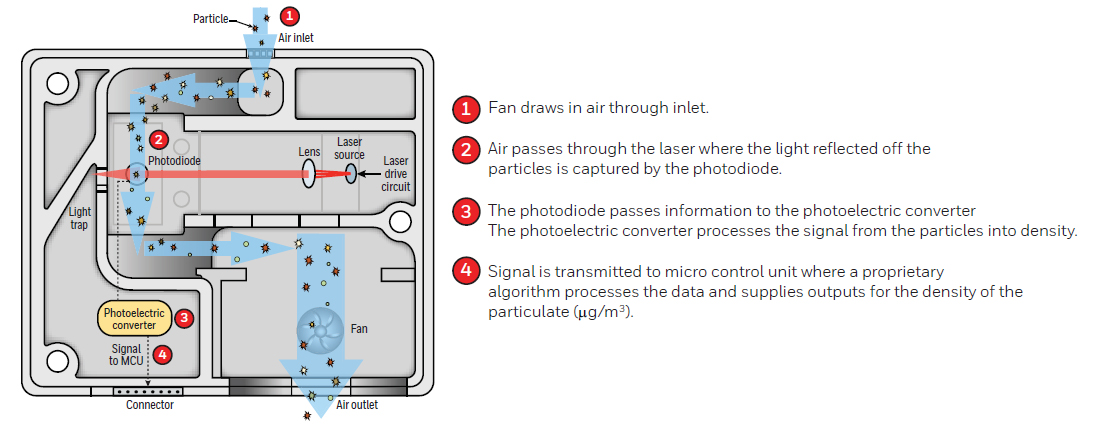
\includegraphics[width=1.00\textwidth]{images/4_SensorSchemiatic}
\caption{Schematic of Honeywell Particulate Matter Sensor. A laser light source illuminates a particle as it is pulled through the detection chamber. As particles pass through the laser beam, the light reflects off the particles and is recorded on the photo or light detector. The light is then analyzed and converted to an electrical signal to calculate particle concentration.}
\label{fig:hpsensor}
\end{figure}

Our sensors can generate several categories of PM data. Using a laser and light defraction, the number and size of the particles can be estimated (Figure~\ref{fig:defraction}).

\begin{figure}
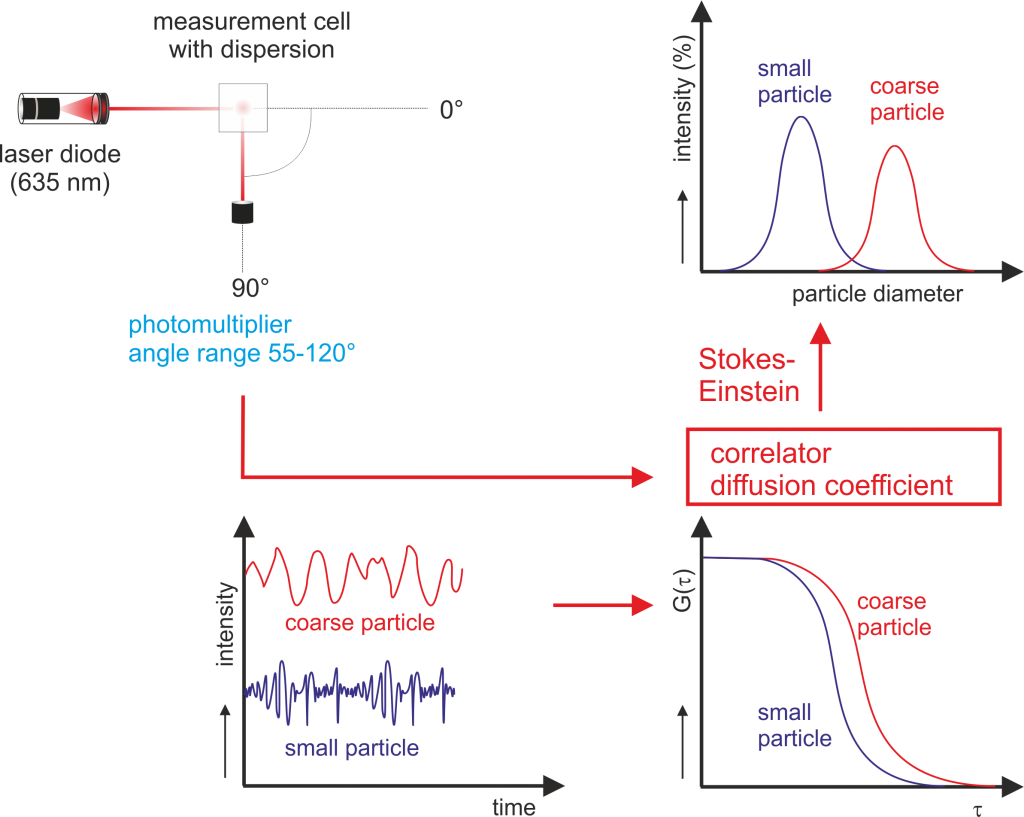
\includegraphics[width=0.70\textwidth]{images/4_Measurement-principle}
\caption{In particle size measurements using light scattering (DLS), a laser beam is scattered on very small, finely dispersed particles in a highly diluted matrix. 
The scattered light of each particle will then interfere with each other. Since the particles constantly change locations, the position of the scattering centers changes with respect to each other and the interferences lead to small fluctuations in scattering intensity (this explains the name ``dynamic'' light scattering).}
\label{fig:defraction}
\end{figure}

\section{Data Collection}
\subsection{What data is collected by the PMS5003?}

The PMS5003 generates the following data: 

\begin{description}
  \item[Data 1] refers to PM1.0 concentration unit $\mu$g/m$^3$(CF=1,standard particle)\footnote{The Asterisk on Data 1 and Data 4 is defined on the same page as ``Note: CF=1 should be used in the factory environment''}
  \item[Data 2] refers to PM2.5 concentration unit $\mu$g/m$^3$(CF=1,standard particle)
  \item[Data 3] refers to PM10 concentration unit $\mu$g/m$^3$(CF=1,standard particle)
  \item[Data 4] refers to PM1.0 concentration unit $\mu$g/m$^3$(under atmospheric environment)
  \item[Data 5] refers to PM2.5 concentration unit $\mu$g/m$^3$(under atmospheric environment)
  \item[Data 6] refers to concentration unit (under atmospheric environment) $\mu$g/m$^3$
  \item[Data 7] indicates the number of particles with diameter beyond 0.3 $\mu$m in 0.1 L of air.
  \item[Data 8] indicates the number of particles with diameter beyond 0.5 $\mu$m in 0.1 L of air.
  \item[Data 9] indicates the number of particles with diameter beyond 1.0 $\mu$m in 0.1 L of air.
  \item[Data 10] indicates the number of particles with diameter beyond 2.5 $\mu$m in 0.1 L of air.
  \item[Data 11] indicates the number of particles with diameter beyond 5.0 $\mu$m in 0.1 L of air.
  \item[Data 12] indicates the number of particles with diameter beyond 10 $\mu$m in 0.1 L of air

\end{description}

The first set are labeled ``standard'', while the second set are labeled ``atmospheric environment''. What do these measure and how do the ``standard'' ones differ from the ``atmospheric environment'' ones?

It has to do with the density of the air used for calculations. "Standard" refers to the concentration ``corrected'' to the ``standard atmosphere'' which in the US is DEFINED as ``having a temperature of 288.15 K at the sea level 0 km geo-potential height and 1013.25 hPa''. NOTE: 288.15 K equals 25 C and Pa are ``pascals'' which is a meausure of pressure. 

On the other hand, the ``ambient conditions'' are just as the air is ``now'' (whatever temperature and pressure there is). Now what does that mean\ldots

Air being a gas, it is compressible which means that it changes its volume when the pressure changes so when you report concentrations as mass per volume of air it is relevant at what pressure that volume is calculated. For example, if you have a bunch of particles rising in the air in a bubble (no loss of particles, no addition, they're just riding a bubble up in the air) then, as they rise, the pressure drops so what was 1cc at the ground it is now 2cc so the concentration of what was in the bubble is now half without anything actually changing other than the ambient pressure. So, it is common to report concentrations (of anything) as ``x mg per standard m3'' and because we scientist don't like to write much (current example excluded) you'll usually see the ``standard'' being dropped because it is ``implicit''.

For gases it is also common to report concentrations as ``parts per million'' or ``ppm'' and that metric is independent of the volume of air as it represents the number of molecules of the gas in a million molecules of air (including the target gas).

In conclusion, I use the ``standard'' readings for reporting but keep the ``ambient conditions'' for analysis. I haven't used these things in high altitudes so for all my deployments the standard and ambient are very similar. I have written code to extract the standard values only -- but you can certain add the ambient if you want to see if there is a difference -- could be important if you are above 1000 ft in elevation.

\section{Collecting the data}

\subsection{Extract Data From Pi}

    Once the data have been collected, you can extract from the Pi -- Unfortunately, there are several ways to do this and NONE of them are easy. 

\subsubsection{For PCs} 
For PCs: Here is \href{https://www.makeuseof.com/tag/copy-data-raspberry-pi-pc/}{webpage that describes the issues and 5 not great options} to get data. 

After several attempts to create a cloud folder that you could upload, I found it was far to slow and unreliable. Thus, I recommend using Putty and the following line commands:

\begin{lstlisting}
psftp> open Pi@XXX.XXX.XXX.XXX
\end{lstlisting}



and you will be prompted to enter the password. Once you are in, you can see your files by entering

\begin{lstlisting}
psftp>ls *.csv
\end{lstlisting}


\noindent where all your csv files should be shown. 

Then you'll need to change your local drive (the default one is write protected, creating a signficant obstacle. So, use 

\begin{lstlisting}
psftp>lpwd
\end{lstlisting}
 

\noindent to see your default directly. We are doing to use the download directory and we can change the directory using:

\begin{lstlisting}
psftp>lcd c:/Downloads
\end{lstlisting}

Then we will get the files...

\begin{lstlisting}
psftp>get airquality_data.csv
\end{lstlisting}


and it will be transfered to your local computer... !  Yay!  It only took me 5 hours to figure out and hopefully for you less than 5 min. 

\subsubsection{FOR Macs}



\subsection{Processing the data}

We create a script to process the data and allow you to create a reasonably user-friendly dataframe to analyze the data.

However, before running the code below, we need to remove all the double quotes, which get in the way of how ``csv'' files are read. 

I opened the document up in rstdudio and did a search for " and replaced with nothing, i.e. don't enter anythning. Then replace all. 

\begin{knitrout}
\definecolor{shadecolor}{rgb}{0.969, 0.969, 0.969}\color{fgcolor}\begin{kframe}
\begin{alltt}
\hlstd{filepath.csv} \hlkwb{=} \hlstr{"/home/CAMPUS/mwl04747/github/EJnPi/data/Air_Quality.csv"}
\hlstd{filepath.csv} \hlkwb{=} \hlstr{"/home/CAMPUS/mwl04747/github/EJnPi/data/Complete_airquality_data.csv"}
\hlstd{rawdata} \hlkwb{=} \hlkwd{read.csv}\hlstd{(filepath.csv)}

\hlkwd{names}\hlstd{(rawdata)}\hlkwb{=} \hlkwd{c}\hlstd{(}\hlstr{"X1"}\hlstd{,} \hlstr{"X2"}\hlstd{,} \hlstr{"Month"}\hlstd{,} \hlstr{"Day"}\hlstd{,} \hlstr{"Hour"}\hlstd{,}
    \hlstr{"Minute"}\hlstd{,} \hlstr{"Second"}\hlstd{,} \hlstr{"X3"}\hlstd{,} \hlstr{"X4"}\hlstd{,} \hlstr{"pm1_cf"}\hlstd{,} \hlstr{"X5"}\hlstd{,} \hlstr{"pm25_cf"}\hlstd{,} \hlstr{"X6"}\hlstd{,}
    \hlstr{"pm10_cf"}\hlstd{,} \hlstr{"X7"}\hlstd{,} \hlstr{"pm1"}\hlstd{,} \hlstr{"X8"}\hlstd{,} \hlstr{"pm25"}\hlstd{,} \hlstr{"pm10."}\hlstd{,} \hlstr{"X9"}\hlstd{)}

\hlstd{rawdata}\hlopt{$}\hlstd{pm1_cf} \hlkwb{=} \hlkwd{as.numeric}\hlstd{(}\hlkwd{gsub}\hlstd{(}\hlstr{'[)]'}\hlstd{,} \hlstr{''}\hlstd{, rawdata}\hlopt{$}\hlstd{pm1_cf))}
\hlstd{rawdata}\hlopt{$}\hlstd{pm25_cf} \hlkwb{=} \hlkwd{as.numeric}\hlstd{(}\hlkwd{gsub}\hlstd{(}\hlstr{'[)]'}\hlstd{,} \hlstr{''}\hlstd{, rawdata}\hlopt{$}\hlstd{pm25_cf))}
\hlstd{rawdata}\hlopt{$}\hlstd{pm10_cf} \hlkwb{=} \hlkwd{as.numeric}\hlstd{(}\hlkwd{gsub}\hlstd{(}\hlstr{'[)]'}\hlstd{,} \hlstr{''}\hlstd{, rawdata}\hlopt{$}\hlstd{pm10_cf))}
\hlkwd{as.Date}\hlstd{(}\hlkwd{with}\hlstd{(rawdata,} \hlkwd{paste}\hlstd{(}\hlstr{"2020"}\hlstd{, Month, Day,}\hlkwc{sep}\hlstd{=}\hlstr{"-"}\hlstd{)),} \hlstr{"%Y-%m-%d"}\hlstd{)[}\hlnum{1}\hlstd{]}
\end{alltt}
\begin{verbatim}
## [1] "2020-10-21"
\end{verbatim}
\begin{alltt}
\hlkwd{library}\hlstd{(lubridate)}
\end{alltt}


{\ttfamily\noindent\itshape\color{messagecolor}{\#\# \\\#\# Attaching package: 'lubridate'}}

{\ttfamily\noindent\itshape\color{messagecolor}{\#\# The following object is masked from 'package:base':\\\#\# \\\#\#\ \ \ \  date}}\begin{alltt}
\hlstd{rawdata}\hlopt{$}\hlstd{DateTime} \hlkwb{=} \hlkwd{with}\hlstd{(rawdata,} \hlkwd{ymd_hms}\hlstd{(}\hlkwd{paste}\hlstd{(}\hlstr{"2020"}\hlstd{, Month,}
  \hlstd{Day, Hour, Minute, Second,} \hlkwc{sep}\hlstd{=} \hlstr{'-'}\hlstd{)))}
\end{alltt}
\end{kframe}
\end{knitrout}

As always, I check my data!

\begin{knitrout}
\definecolor{shadecolor}{rgb}{0.969, 0.969, 0.969}\color{fgcolor}\begin{kframe}
\begin{alltt}
\hlkwd{head}\hlstd{(rawdata)[}\hlnum{1}\hlstd{]}
\end{alltt}
\begin{verbatim}
##                         X1
## 1 OrderedDict([('DateTime'
## 2 OrderedDict([('DateTime'
## 3 OrderedDict([('DateTime'
## 4 OrderedDict([('DateTime'
## 5 OrderedDict([('DateTime'
## 6 OrderedDict([('DateTime'
\end{verbatim}
\begin{alltt}
\hlcom{# Remove Variables}
\hlstd{cleandata} \hlkwb{=} \hlkwd{subset}\hlstd{(rawdata,} \hlkwc{select}\hlstd{=}\hlkwd{c}\hlstd{(DateTime, pm1_cf, pm25_cf, pm10_cf))}
\end{alltt}
\end{kframe}
\end{knitrout}

\subsection{Plot Data}

As usual, it's a good idea to get a sense of the variability of the data. 
\begin{knitrout}
\definecolor{shadecolor}{rgb}{0.969, 0.969, 0.969}\color{fgcolor}\begin{kframe}
\begin{alltt}
\hlkwd{hist}\hlstd{(cleandata}\hlopt{$}\hlstd{pm25_cf,} \hlkwc{xlab}\hlstd{=}\hlstr{"PM2.5 concentration"}\hlstd{,}
    \hlkwc{main}\hlstd{=}\hlstr{"Histogram of PM2.5 in Claremont"}\hlstd{,} \hlkwc{las}\hlstd{=}\hlnum{1}\hlstd{,} \hlkwc{xlim}\hlstd{=}\hlkwd{c}\hlstd{(}\hlnum{0}\hlstd{,}\hlnum{100}\hlstd{))}
\end{alltt}
\end{kframe}
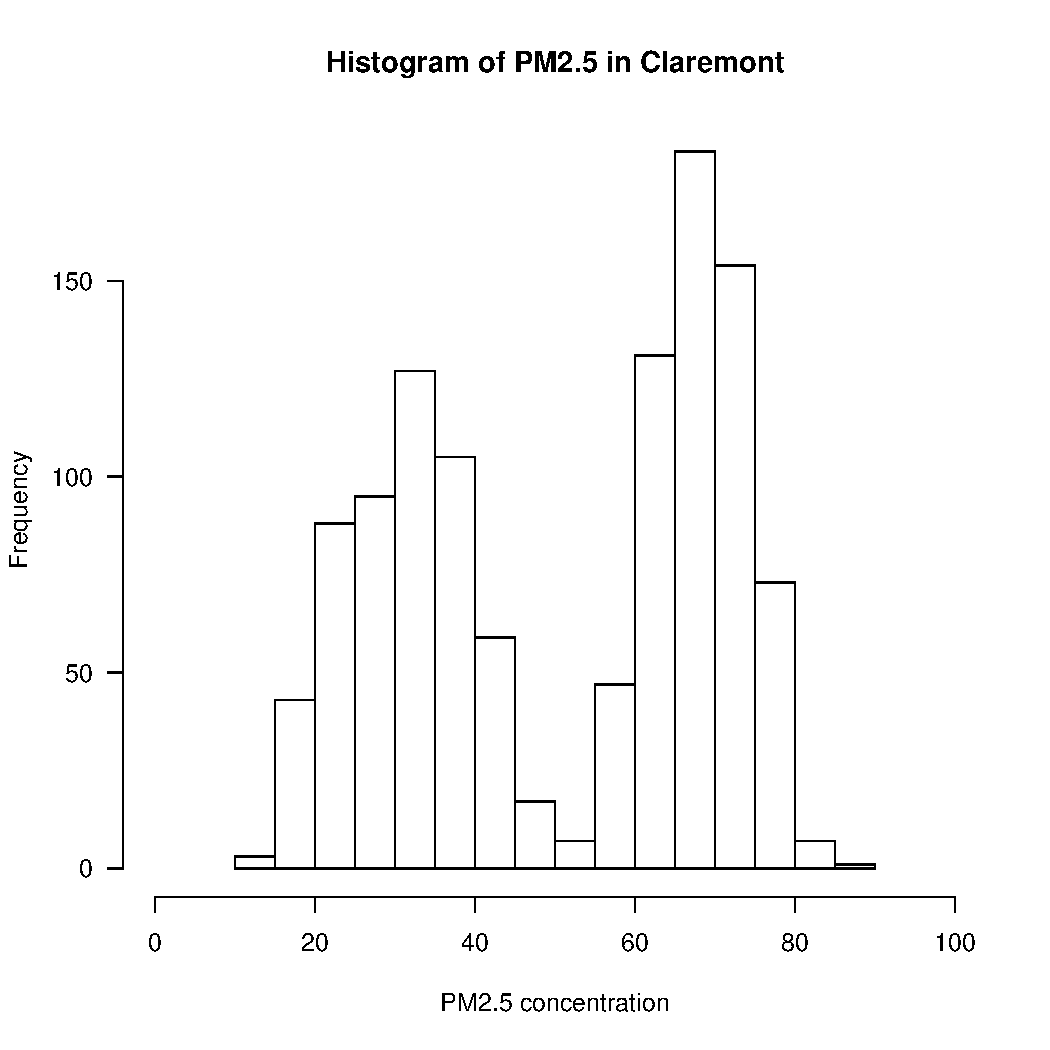
\includegraphics[width=\maxwidth]{figure/unnamed-chunk-3-1} 

\end{knitrout}

In my case, I have a very odd bimodal distribution. So, I am going plot on a time series to see if I can figure out what in the world is going on.

\begin{knitrout}
\definecolor{shadecolor}{rgb}{0.969, 0.969, 0.969}\color{fgcolor}\begin{kframe}
\begin{alltt}
\hlkwd{plot}\hlstd{(pm25_cf}\hlopt{~}\hlstd{DateTime,} \hlkwc{data}\hlstd{=cleandata,} \hlkwc{pch}\hlstd{=}\hlnum{20}\hlstd{,} \hlkwc{cex}\hlstd{=}\hlnum{.5}\hlstd{)}
\end{alltt}
\end{kframe}
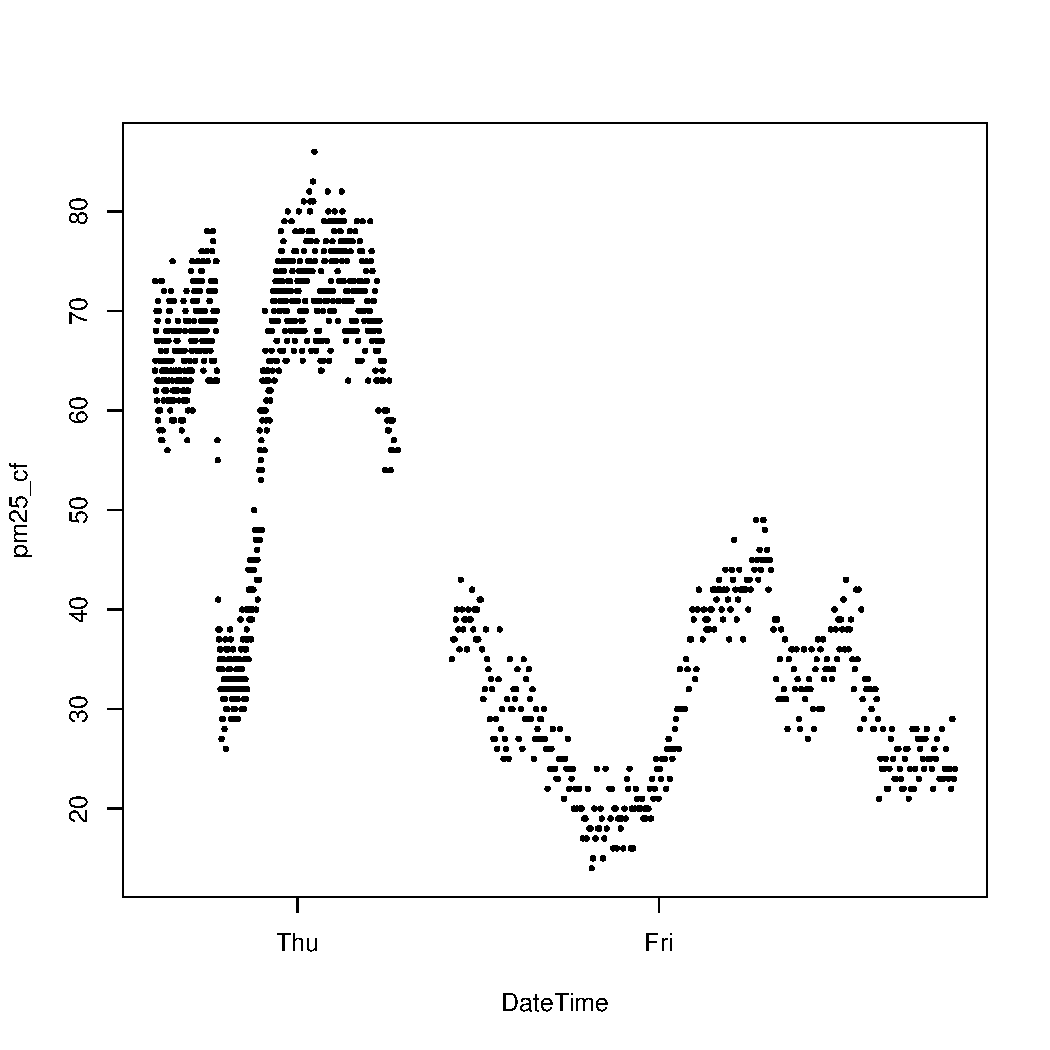
\includegraphics[width=\maxwidth]{figure/unnamed-chunk-4-1} 

\end{knitrout}

Except for some breaks in the data, we can certainly see a diurnal pattern, where the concentrations seem highest after midnight. 

Let's see if we can add times to the plot!

\begin{knitrout}
\definecolor{shadecolor}{rgb}{0.969, 0.969, 0.969}\color{fgcolor}\begin{kframe}
\begin{alltt}
\hlkwd{plot}\hlstd{(pm25_cf}\hlopt{~}\hlstd{DateTime,} \hlkwc{data}\hlstd{=cleandata,} \hlkwc{pch}\hlstd{=}\hlnum{20}\hlstd{,}
    \hlkwc{cex}\hlstd{=}\hlnum{.5}\hlstd{,} \hlkwc{las}\hlstd{=}\hlnum{1}\hlstd{,} \hlkwc{ylab}\hlstd{=}\hlstr{"PM2.5"}\hlstd{,} \hlkwc{xlab}\hlstd{=}\hlstr{"Time"}\hlstd{,}
    \hlkwc{ylim}\hlstd{=}\hlkwd{c}\hlstd{(}\hlnum{0}\hlstd{,}\hlnum{90}\hlstd{),} \hlkwc{xaxt}\hlstd{=}\hlstr{'n'}\hlstd{)}
\hlkwd{library}\hlstd{(Hmisc)}
\end{alltt}


{\ttfamily\noindent\itshape\color{messagecolor}{\#\# Loading required package: lattice}}

{\ttfamily\noindent\itshape\color{messagecolor}{\#\# Loading required package: survival}}

{\ttfamily\noindent\itshape\color{messagecolor}{\#\# Loading required package: Formula}}

{\ttfamily\noindent\itshape\color{messagecolor}{\#\# Loading required package: ggplot2}}

{\ttfamily\noindent\itshape\color{messagecolor}{\#\# \\\#\# Attaching package: 'Hmisc'}}

{\ttfamily\noindent\itshape\color{messagecolor}{\#\# The following objects are masked from 'package:base':\\\#\# \\\#\#\ \ \ \  format.pval, units}}\begin{alltt}
\hlcom{#minor.tick(nx=4, tick.ratio=1)}
\hlcom{#axis.lab=c(as.Date(c("2020-10-20", "2020-10-21", "2020-10-24")))}
\hlkwd{axis}\hlstd{(}\hlnum{1}\hlstd{, cleandata}\hlopt{$}\hlstd{DateTime,} \hlkwd{format}\hlstd{(cleandata}\hlopt{$}\hlstd{DateTime,} \hlstr{"%H"}\hlstd{),} \hlkwc{cex.axis} \hlstd{=} \hlnum{.7}\hlstd{,}  \hlkwc{tck}\hlstd{=}\hlopt{-}\hlnum{.05}\hlstd{)}

\hlkwd{axis}\hlstd{(}\hlnum{3}\hlstd{, cleandata}\hlopt{$}\hlstd{DateTime,} \hlkwd{format}\hlstd{(cleandata}\hlopt{$}\hlstd{DateTime,} \hlstr{"%a"}\hlstd{),} \hlkwc{cex.axis} \hlstd{=} \hlnum{.7}\hlstd{,}  \hlkwc{tck}\hlstd{=}\hlnum{0}\hlstd{)}\hlcom{#, at=axis.lab, labels=axis.lab)}
\end{alltt}
\end{kframe}
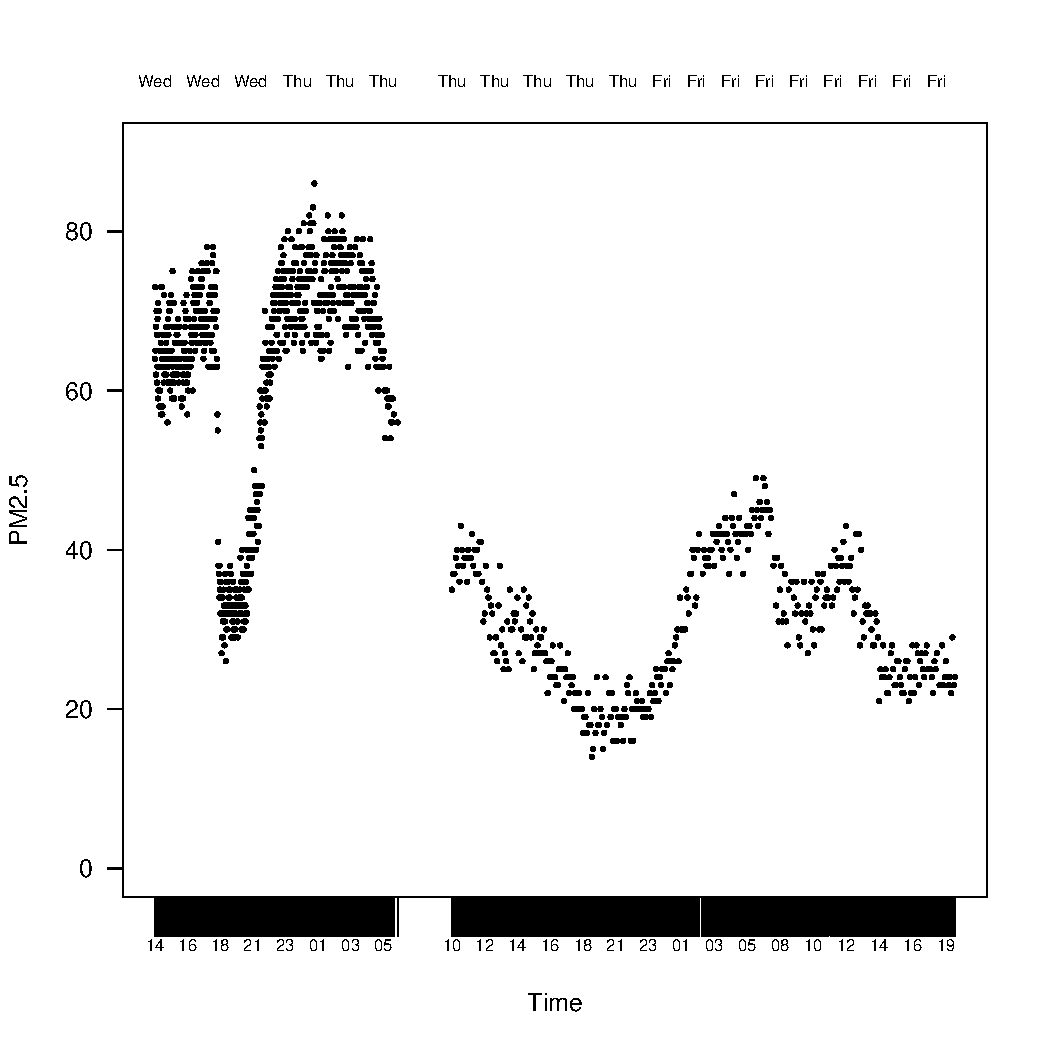
\includegraphics[width=\maxwidth]{figure/unnamed-chunk-5-1} 
\begin{kframe}\begin{alltt}
\hlcom{#axis.Date(1,at=cleandata$DateTime,labels=format(cleandata$DateTime,"%H"),las=1)}
\end{alltt}
\end{kframe}
\end{knitrout}

Not perfect, but good enough -- sows a that Claremont's Air Quality was terrible on Wednesday night and Thursday morning. 

\section{Comparing Data to EPA Stations}

\subsection{Using previous collected data}

\begin{knitrout}
\definecolor{shadecolor}{rgb}{0.969, 0.969, 0.969}\color{fgcolor}\begin{kframe}
\begin{alltt}
\hlcom{# TBD}
\end{alltt}
\end{kframe}
\end{knitrout}

\subsection{Comparing $\mu$ to EPA Data}

The population mean (monthly average from the EPA data) is a parameter estimate. We can determine if the values you collected fall within the parameter estimate and it's 95\% confidence intervals. 


\subsection{More Intricate Analysis}

You could look to see if the there is a different during the time of the day or day of the week. You could move you sensor around in and outside your house and see if air quality is better / worse or the same\ldots.

We can help you with r code if you'd like to follow up with these additional questions. 


\end{document}
